% Source: graduate-coursework/Prior_Semesters/Fa25/EMCH501/HW3/HW3.tex
% Description: Schematic of the 1D heat equation problem with mixed boundary conditions.

\documentclass[border=4pt]{standalone}
\usepackage{amsmath}
\usepackage{amssymb}
\usepackage{graphicx}
\usepackage{pgfplots}
\usepackage{tikz}
\usepackage{xcolor}
\pgfplotsset{compat=1.18}
\usetikzlibrary{shapes.geometric, arrows.meta, positioning, decorations.pathmorphing, patterns}

\definecolor{USC_Garnet}{HTML}{73000A}
\definecolor{USC_Sandstorm}{HTML}{FFF2E3}
\definecolor{USC_Black90}{HTML}{565656}
\definecolor{USC_Black10}{HTML}{ECECEC}
\definecolor{USC_Honeycomb}{HTML}{65780B}

\begin{document}
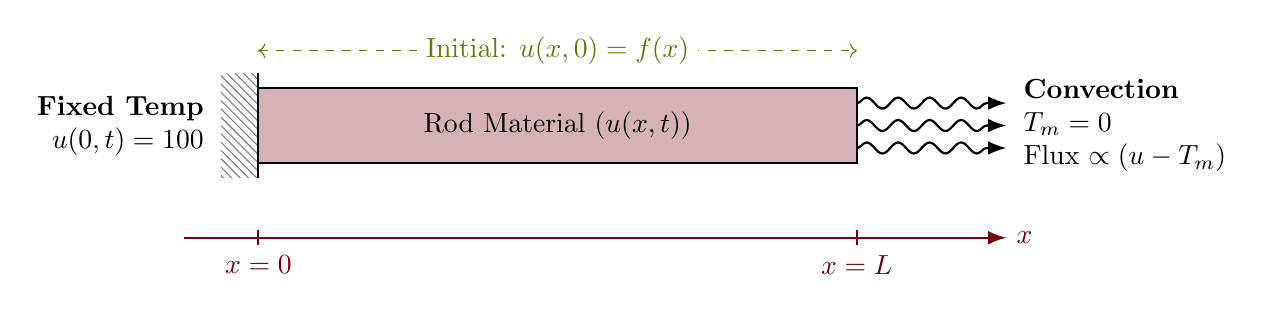
\begin{tikzpicture}[scale=0.95]
        % Parameters
        \def\RodLen{8}
        \def\RodH{1}
        
        % 1. Draw the Axis
        \draw[-Latex, thick, USC_Garnet] (-1, -1) -- (\RodLen + 2, -1) node[right] {$x$};
        
        % Ticks and labels
        \draw[thick, USC_Garnet] (0, -0.9) -- (0, -1.1) node[below] {$x=0$};
        \draw[thick, USC_Garnet] (\RodLen, -0.9) -- (\RodLen, -1.1) node[below] {$x=L$};
        
        % 2. Draw the Rod
        \draw[fill=USC_Garnet!30, thick] (0,0) rectangle (\RodLen, \RodH);
        \node at (\RodLen/2, \RodH/2) {Rod Material ($u(x,t)$)};
        
        % 3. Left Boundary Condition (Fixed Temp)
        \fill[pattern=north west lines, pattern color=gray] (-0.5, -0.2) rectangle (0, \RodH + 0.2);
        \draw[thick] (0, -0.2) -- (0, \RodH + 0.2);
        
        % Label for Left BC
        \node[anchor=east, align=right] at (-0.6, \RodH/2) {
            \textbf{Fixed Temp}\\
            $u(0,t) = 100$
        };
        
        % 4. Right Boundary Condition (Convection)
        \foreach \y in {0.2, 0.5, 0.8} {
            \draw[-Latex, thick, decorate, decoration={snake, amplitude=0.7mm, segment length=4mm, post length=2mm}] 
            (\RodLen, \y) -- (\RodLen + 2.0, \y);
        }
        
        % Label for Right BC
        \node[anchor=west, align=left] at (\RodLen + 2.1, \RodH/2) {
            \textbf{Convection}\\
            $T_m = 0$\\
            Flux $\propto (u - T_m)$
        };
        
        % 5. Initial Condition Label
        \draw[<->, dashed, USC_Honeycomb] (0, \RodH + 0.5) -- (\RodLen, \RodH + 0.5) node[midway, fill=white] {Initial: $u(x,0) = f(x)$};

    \end{tikzpicture}
\end{document}
